\documentclass[aspectratio=169,11pt]{beamer}

\usetheme{Madrid}
\usecolortheme{default}
\setbeamertemplate{navigation symbols}{}
\setbeamertemplate{footline}[frame number]

\usepackage[utf8]{inputenc}
\usepackage[T1]{fontenc}
\usepackage{graphicx}
\usepackage{booktabs}
\usepackage{tabularx}
\usepackage{array}
\usepackage{xcolor}

\graphicspath{{../evaluation/}}

\definecolor{PulsarideBlue}{RGB}{16,42,67}
\definecolor{PulsarideTeal}{RGB}{15,118,110}
\definecolor{PulsarideGreen}{RGB}{21,128,61}
\definecolor{PulsarideAmber}{RGB}{180,83,9}
\definecolor{PulsarideRed}{RGB}{180,35,24}

\setbeamercolor{title}{fg=white,bg=PulsarideBlue}
\setbeamercolor{frametitle}{fg=white,bg=PulsarideBlue}
\setbeamercolor{structure}{fg=PulsarideTeal}
\setbeamercolor{block title}{fg=white,bg=PulsarideBlue}
\setbeamercolor{block body}{fg=black,bg=gray!7}

\newcommand{\metric}[2]{\textbf{#1}\\{\small #2}}
\newcommand{\statusdone}{\textcolor{PulsarideGreen}{\textbf{Done}}}
\newcommand{\statuslimit}{\textcolor{PulsarideAmber}{\textbf{Limit}}}

\title[Pulsaride Dispatch Engine]{Pulsaride Medical Dispatch Engine}
\subtitle{V1 Spring Boot API, evaluation, and live dashboard}
\author[S. Sossey \& I. Ben Labsir]{Salmane Sossey \and Ihssan Ben Labsir}
\institute[Pulsaride Solutions]{Internship project supervised by M. Lyazid Salihi\\Pulsaride Solutions}
\date{Oral defense}

\begin{document}

\begin{frame}
  \titlepage
\end{frame}

\begin{frame}{Executive Summary}
  \begin{columns}[T]
    \begin{column}{0.52\textwidth}
      \begin{block}{Problem}
        Medical requests must be assigned quickly to available professionals, while keeping the process auditable and measurable.
      \end{block}
      \begin{block}{Delivered V1}
        A runnable dispatch engine with Spring Boot, PostgreSQL, Redis, Python evaluation scripts, Docker Compose, and a live dashboard.
      \end{block}
    \end{column}
    \begin{column}{0.42\textwidth}
      \begin{block}{Key V1 outcome}
        \begin{itemize}
          \item Full request lifecycle implemented
          \item Four dispatch strategies compared
          \item Robustness and load tested
          \item Honest limits documented
        \end{itemize}
      \end{block}
    \end{column}
  \end{columns}
\end{frame}

\begin{frame}{Project Scope}
  \begin{columns}[T]
    \begin{column}{0.48\textwidth}
      \begin{block}{Functional scope}
        \begin{itemize}
          \item Create and prioritize patient requests
          \item Search available professional slots
          \item Reserve, propose, accept, refuse, timeout, close
          \item Keep assignment history and state transitions
          \item Expose operational metrics
        \end{itemize}
      \end{block}
    \end{column}
    \begin{column}{0.48\textwidth}
      \begin{block}{Engineering scope}
        \begin{itemize}
          \item Spring Boot API
          \item PostgreSQL persistence and audit
          \item Redis queue and locking
          \item Docker Compose execution
          \item Python simulation and evaluation
        \end{itemize}
      \end{block}
    \end{column}
  \end{columns}
\end{frame}

\begin{frame}{Architecture V1}
  \begin{block}{Runtime view}
    \begin{tabularx}{\textwidth}{>{\bfseries}l X}
      API & Spring Boot exposes requests, dispatch, availability, metrics, AI mock triage, and dashboard endpoints.\\
      PostgreSQL & Stores professionals, requests, slots, assignments, and state transitions for audit and evaluation.\\
      Redis & Coordinates real-time queueing and slot/request locks to avoid duplicate assignment.\\
      Python evaluator & Loads scenarios, drives the live API, computes metrics, and generates charts.\\
      Docker Compose & Starts PostgreSQL, Redis, and the API in one reproducible environment.
    \end{tabularx}
  \end{block}

  \vspace{0.2cm}
  \begin{center}
    \small Patient request $\rightarrow$ Redis priority queue $\rightarrow$ Dispatch strategy $\rightarrow$ Slot reservation $\rightarrow$ Professional response $\rightarrow$ PostgreSQL audit
  \end{center}
\end{frame}

\begin{frame}{Dispatch Lifecycle}
  \begin{block}{Finite-state workflow}
    \begin{center}
      \Large
      PENDING $\rightarrow$ RESERVED $\rightarrow$ PROPOSED $\rightarrow$ ACCEPTED $\rightarrow$ CLOSED
    \end{center}
  \end{block}

  \begin{columns}[T]
    \begin{column}{0.48\textwidth}
      \begin{block}{Refusal or timeout}
        \begin{center}
          PROPOSED $\rightarrow$ REFUSED/FAILED $\rightarrow$ PENDING
        \end{center}
        The request returns to the queue and can be reassigned.
      \end{block}
    \end{column}
    \begin{column}{0.48\textwidth}
      \begin{block}{Auditability}
        Each assignment attempt and each state transition is persisted, so the demo can explain what happened and why.
      \end{block}
    \end{column}
  \end{columns}
\end{frame}

\begin{frame}{Availability Service}
  \begin{block}{Why availability is separated from profile data}
    Professional profile data is stable, while availability is operational and changes during dispatch. V1 stores slots separately so matching can search active availability efficiently.
  \end{block}

  \begin{columns}[T]
    \begin{column}{0.5\textwidth}
      \begin{itemize}
        \item AVAILABLE: can receive a proposal
        \item RESERVED: selected and locked for one request
        \item BUSY: accepted consultation in progress
      \end{itemize}
    \end{column}
    \begin{column}{0.5\textwidth}
      \begin{itemize}
        \item BREAK: unavailable after refusal or timeout
        \item OFFLINE: manually unavailable
        \item Redis mirrors active slots and locks selected slots
      \end{itemize}
    \end{column}
  \end{columns}
\end{frame}

\begin{frame}{Dispatch Strategies}
  \begin{tabularx}{\textwidth}{>{\bfseries}l l X}
    \toprule
    ID & Name & Decision rule\\
    \midrule
    S1 & Round Robin & Rotates between currently available slots using the last S1 assignment history.\\
    S2 & Tag Exact & Requires exact specialty match; useful to expose no-availability cases.\\
    S3 & Score Composite & Combines specialty affinity, availability, and professional load.\\
    S4 & Lexical IA & Adds deterministic lexical similarity between patient text and professional profile.\\
    \bottomrule
  \end{tabularx}

  \vspace{0.35cm}
  \begin{block}{Decision for V1}
    S3/S4 are the recommended operational strategies; S1 is useful as a fairness baseline and S2 as a strict matching baseline.
  \end{block}
\end{frame}

\begin{frame}{Strategy Comparison Results}
  \begin{columns}[T]
    \begin{column}{0.48\textwidth}
      \begin{tabular}{lrrrr}
        \toprule
        Strategy & Service & TTFA & TTR & Gini\\
        \midrule
        S1 & 100\% & 4 924 & 5 037 & 0.54\\
        S2 & 90\% & 3 184 & 3 265 & 0.43\\
        S3 & 100\% & 3 188 & 3 282 & 0.27\\
        S4 & 100\% & 3 044 & 3 129 & 0.26\\
        \bottomrule
      \end{tabular}
      \vspace{0.25cm}

      \small Metrics are produced from the live Spring Boot API with 20 requests, 20 professionals, and fixed seed 42.
    \end{column}
    \begin{column}{0.48\textwidth}
      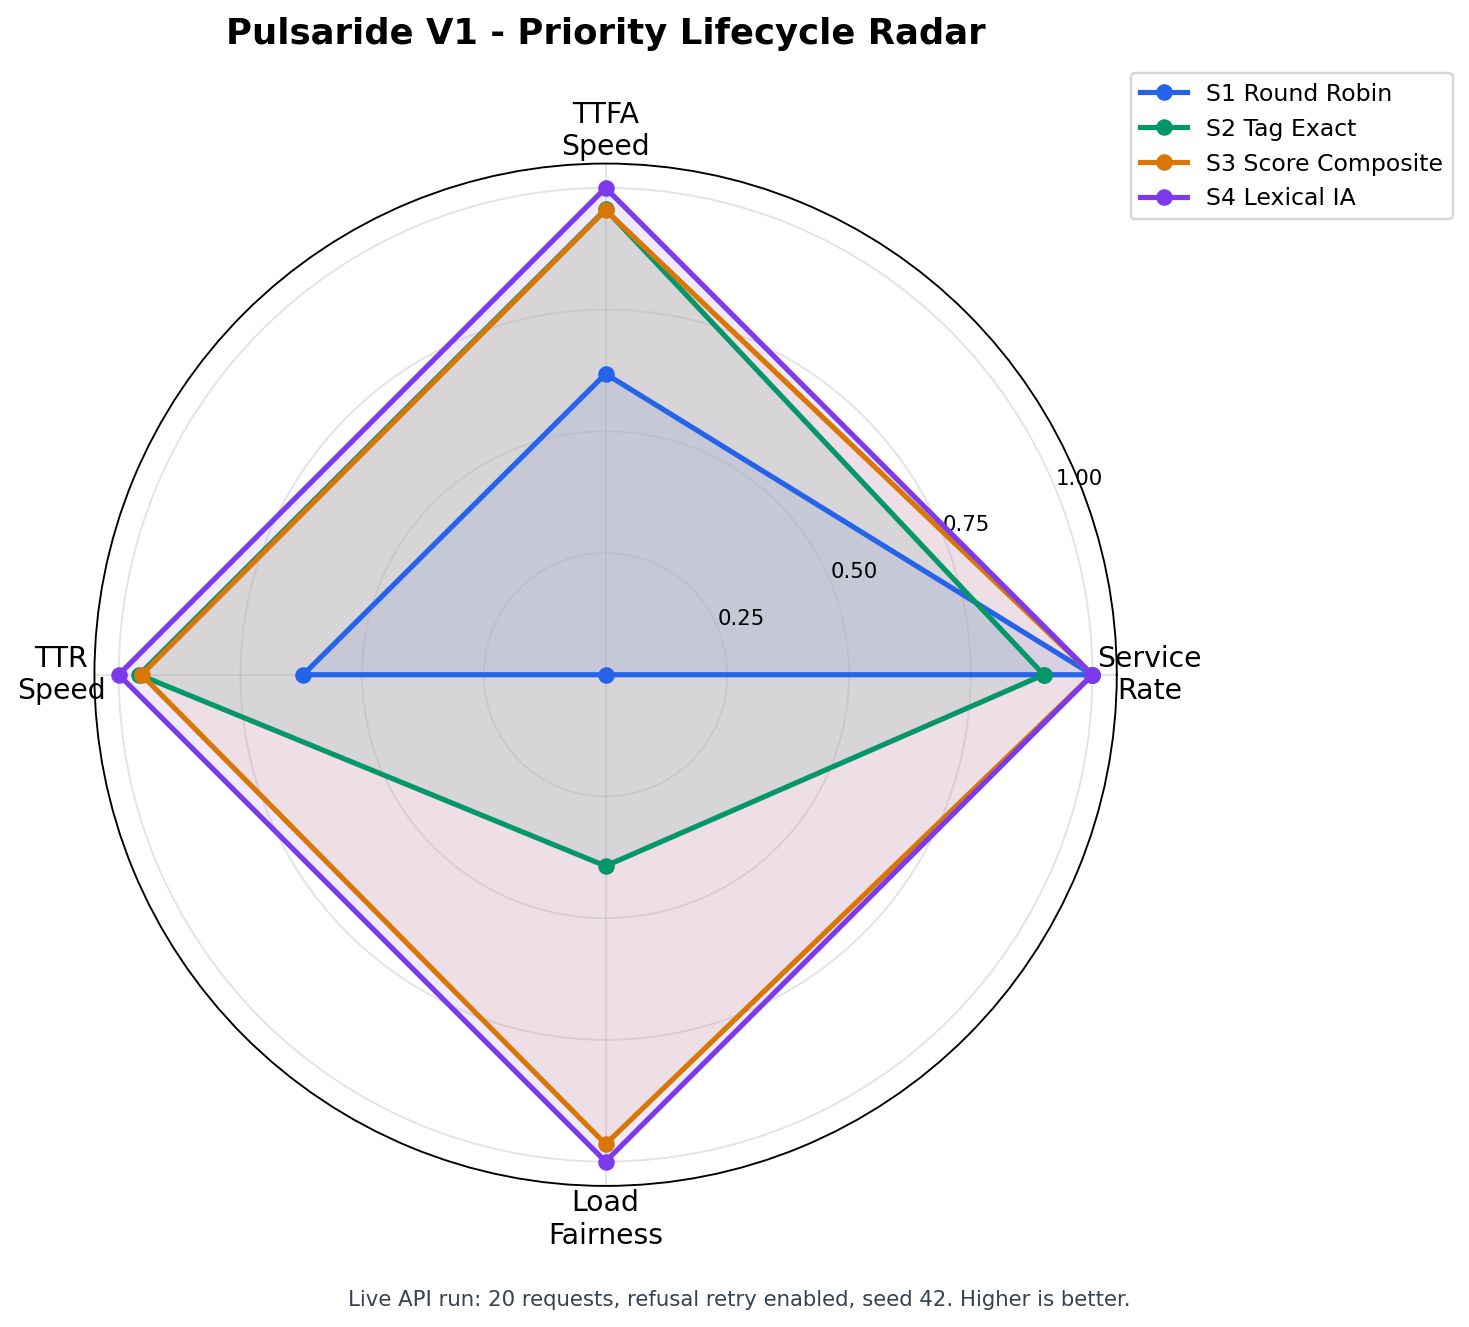
\includegraphics[width=\textwidth]{radar_chart.png}
    \end{column}
  \end{columns}
\end{frame}

\begin{frame}{Comparison Charts}
  \begin{center}
    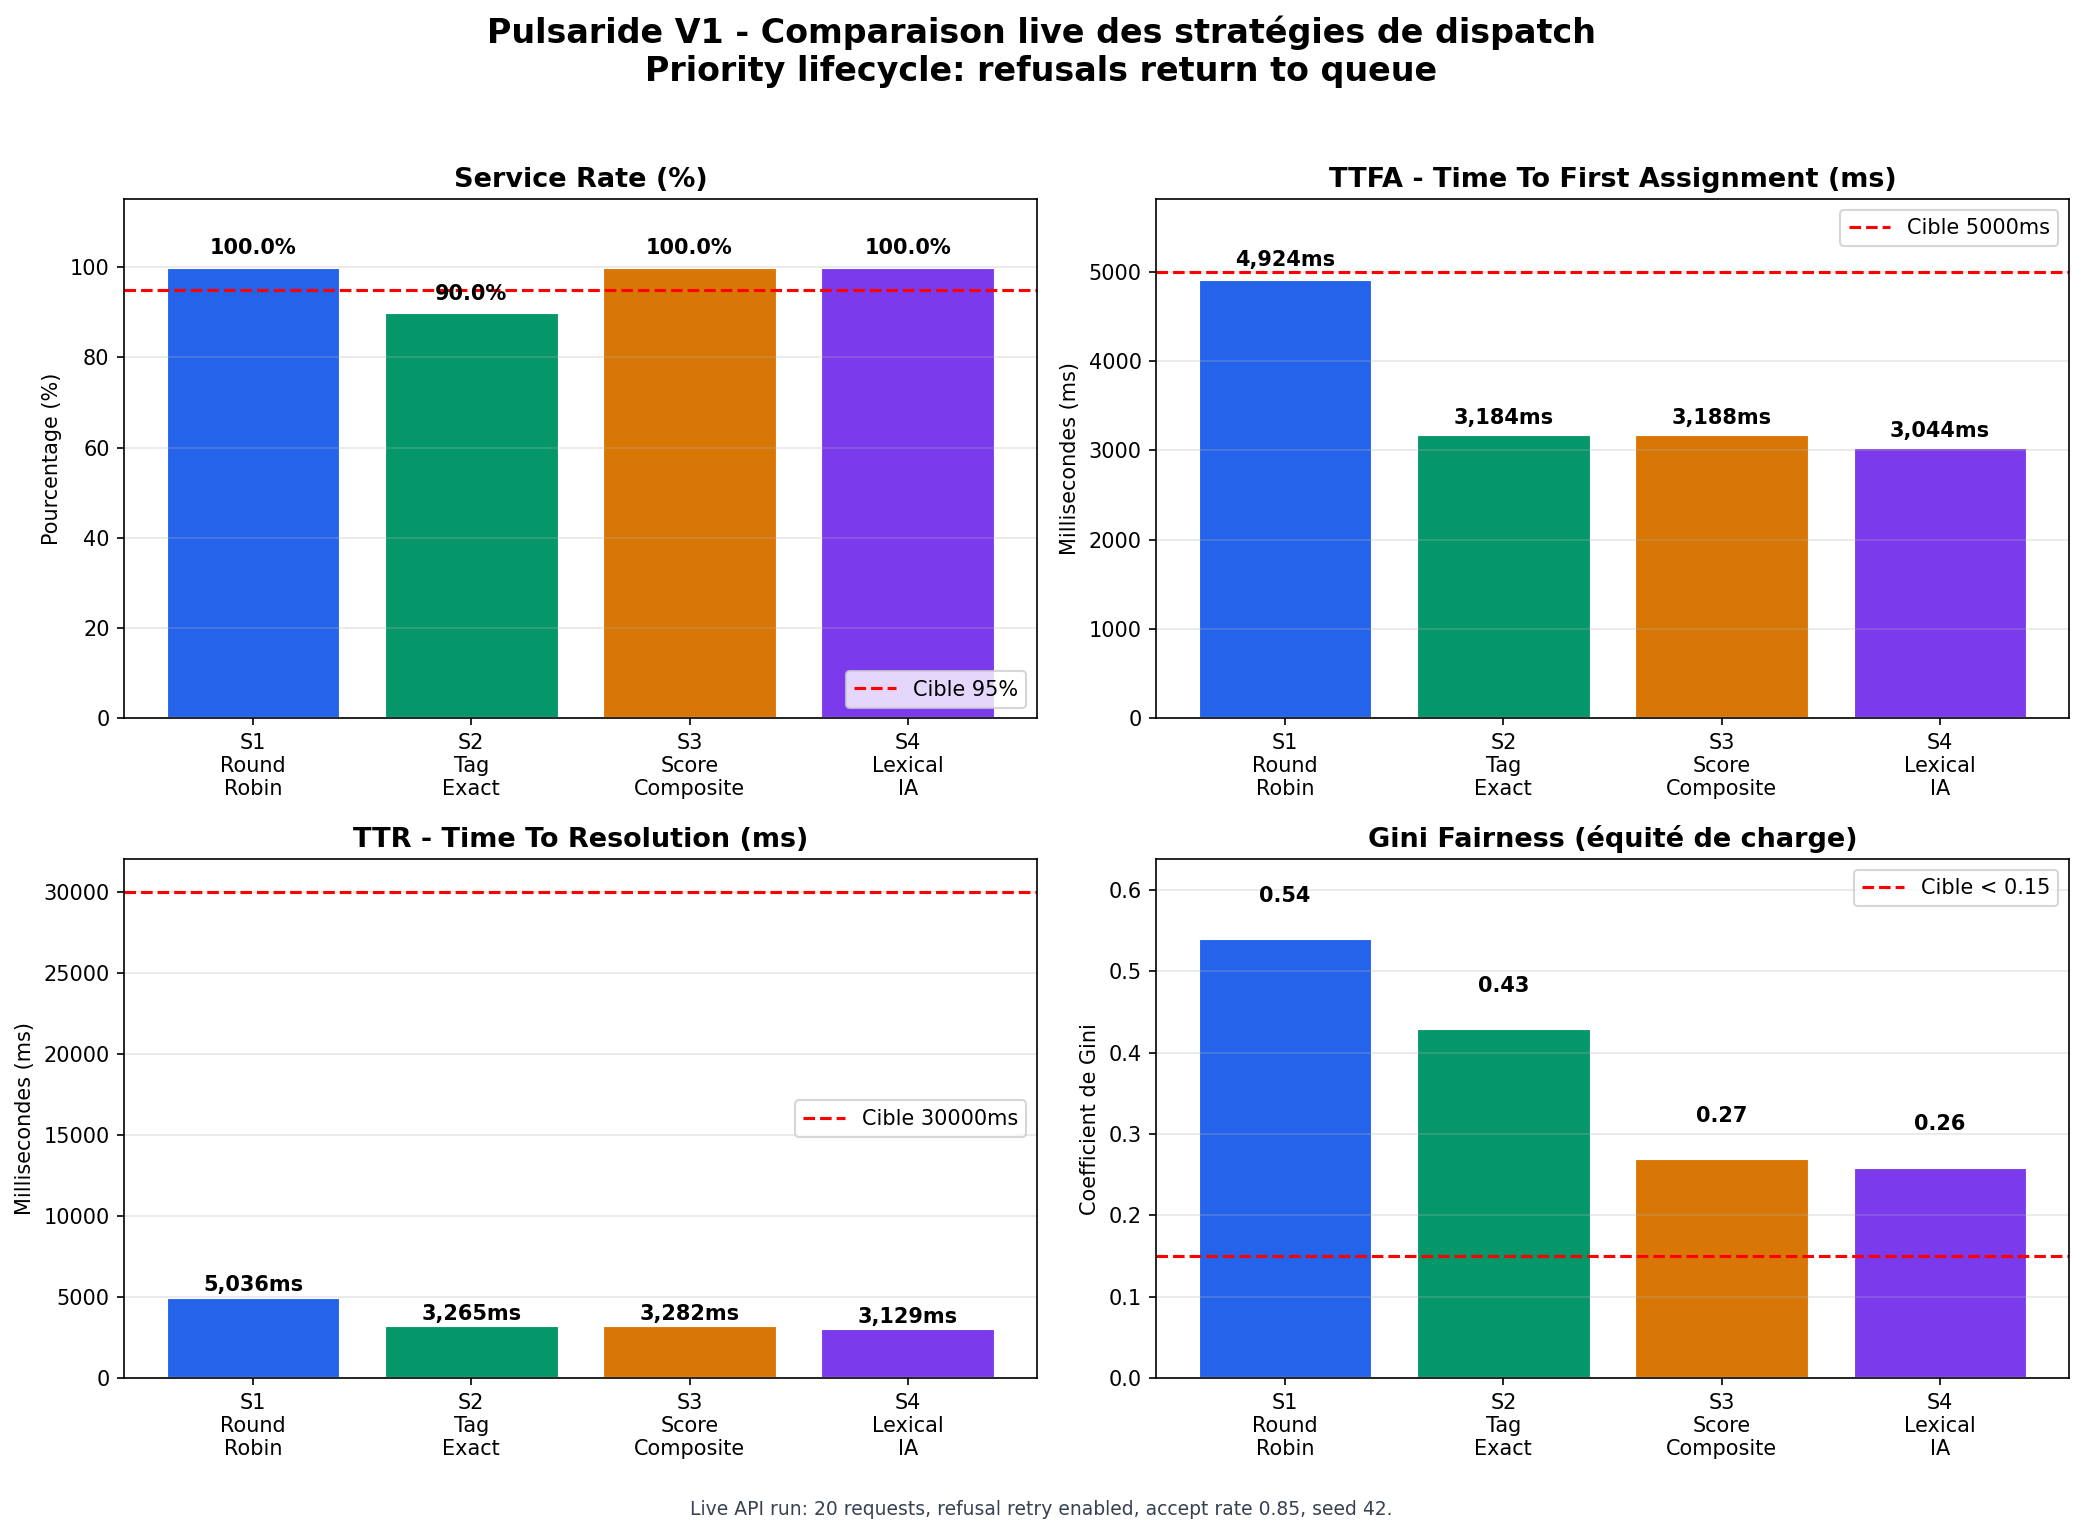
\includegraphics[height=0.76\textheight,keepaspectratio]{comparison_charts.png}
  \end{center}
\end{frame}

\begin{frame}{Robustness and Load Evaluation}
  \begin{columns}[T]
    \begin{column}{0.46\textwidth}
      \begin{block}{Latest P4 rerun}
        \begin{itemize}
          \item Strategy tested: S3
          \item Max sustainable load: 20 requests
          \item Max sustainable throughput: 18.45 closed/s
          \item First degraded load: 40 requests
        \end{itemize}
      \end{block}
      \begin{block}{Reason for degradation}
        At 40 requests, service rate drops to 90\% because some requests remain PENDING inside the test timeout window.
      \end{block}
    \end{column}
    \begin{column}{0.5\textwidth}
      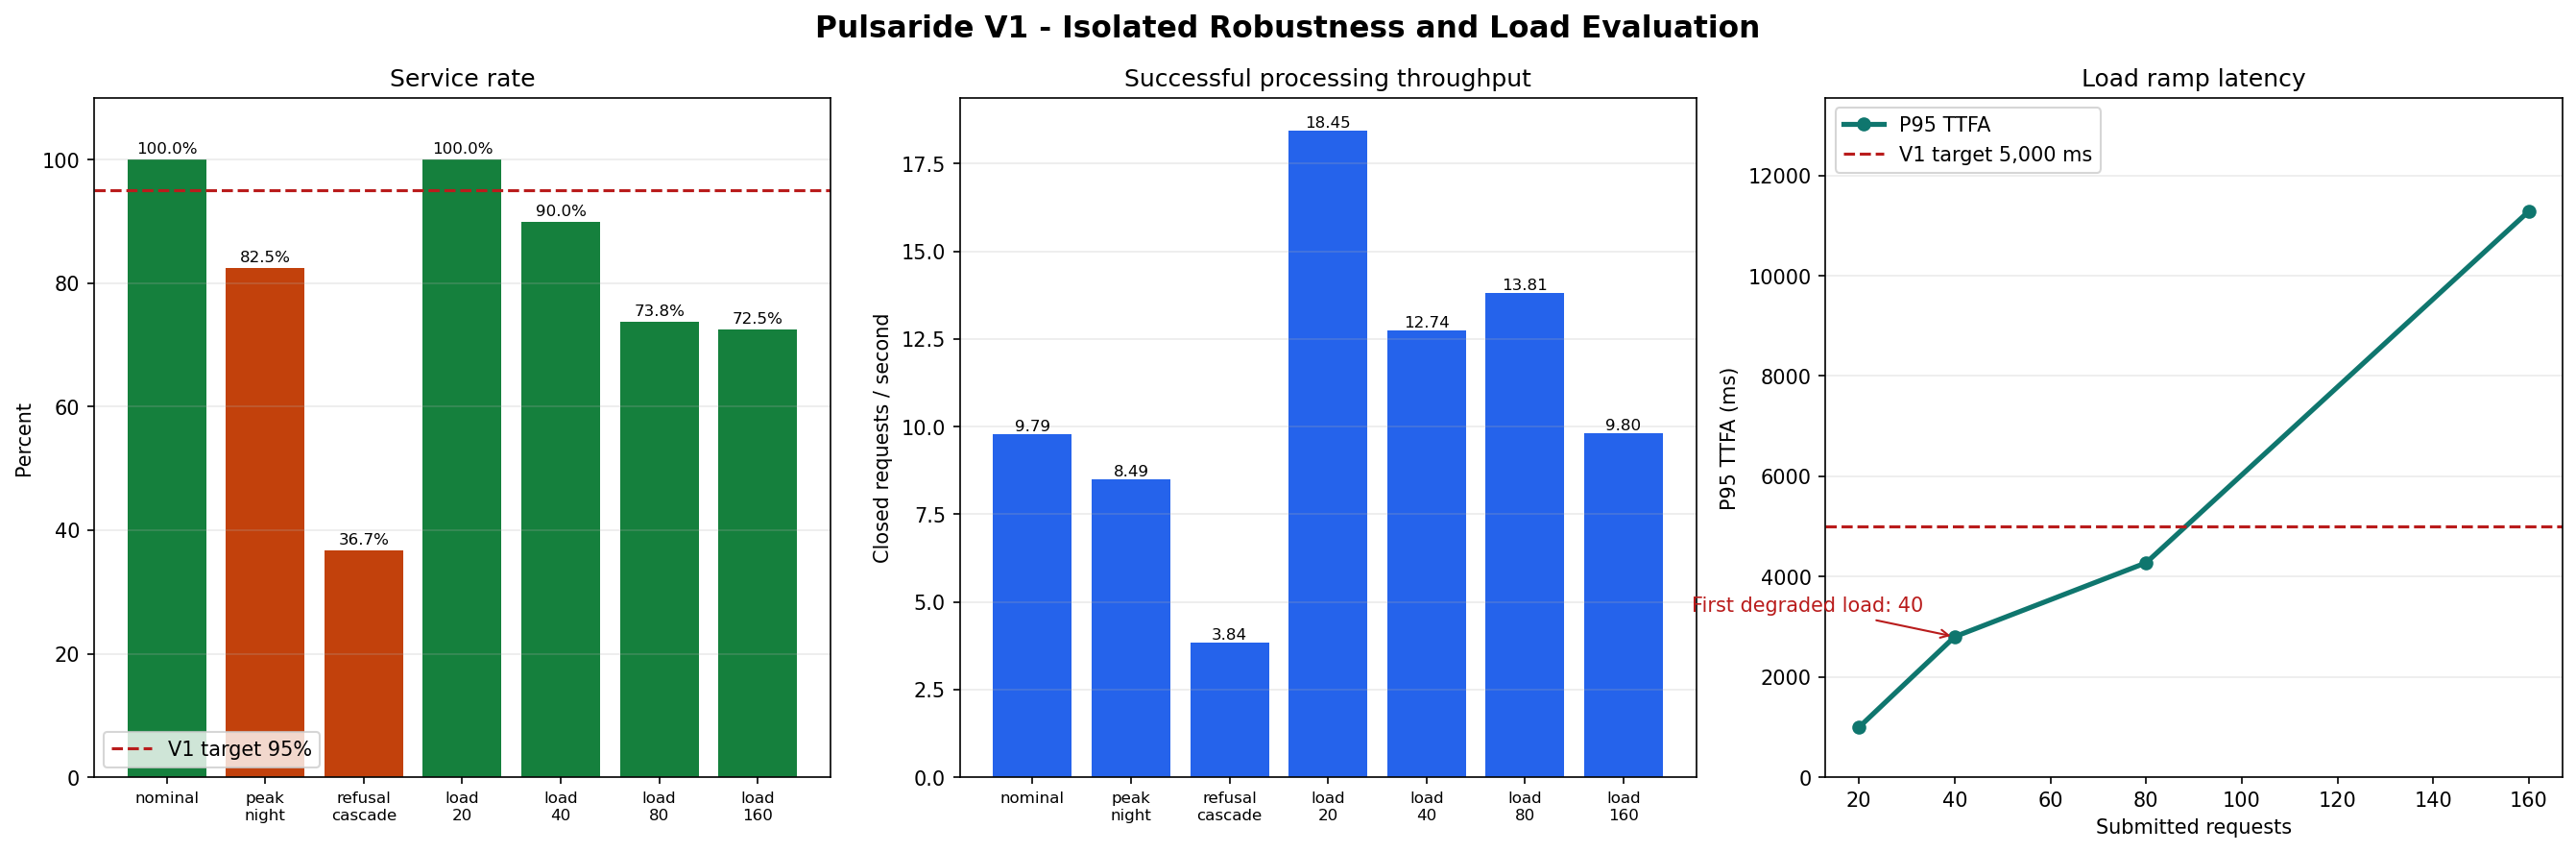
\includegraphics[width=\textwidth]{robustness_charts.png}
    \end{column}
  \end{columns}
\end{frame}

\begin{frame}{Operational Dashboard}
  \begin{block}{Delivered dashboard}
    The dashboard is served directly by Spring Boot at \texttt{/dashboard.html}, so no additional frontend service is needed for the V1 demo.
  \end{block}

  \begin{columns}[T]
    \begin{column}{0.48\textwidth}
      \begin{itemize}
        \item Live KPIs: service rate, TTFA/TTR P95, Gini
        \item Request flow by status
        \item Availability by specialty
      \end{itemize}
    \end{column}
    \begin{column}{0.48\textwidth}
      \begin{itemize}
        \item Professional status and load
        \item Auto-refresh every 5 seconds
        \item Uses existing API endpoints
      \end{itemize}
    \end{column}
  \end{columns}

  \vspace{0.3cm}
  \begin{center}
    \texttt{http://localhost:8080/dashboard.html}
  \end{center}
\end{frame}

\begin{frame}{Quality and Verification}
  \begin{columns}[T]
    \begin{column}{0.5\textwidth}
      \begin{block}{Automated checks}
        \begin{itemize}
          \item Spring Boot test suite passed
          \item 14 tests, 0 failures
          \item Round-robin regression test added
          \item API integration tests cover lifecycle and metrics
        \end{itemize}
      \end{block}
    \end{column}
    \begin{column}{0.46\textwidth}
      \begin{block}{Runtime checks}
        \begin{itemize}
          \item Docker containers healthy
          \item Dashboard returns HTTP 200
          \item Evaluation scripts run against real API
          \item Charts and JSON reports are versioned
        \end{itemize}
      \end{block}
    \end{column}
  \end{columns}
\end{frame}

\begin{frame}{Limits and Honest Interpretation}
  \begin{block}{Known V1 limits}
    \begin{itemize}
      \item Gini fairness remains above the ideal target of 0.15.
      \item Concurrency increases Redis lock contention during high load.
      \item BREAK slots do not yet return automatically to AVAILABLE.
      \item S4 is deterministic lexical matching, not a real embedding model yet.
    \end{itemize}
  \end{block}

  \begin{block}{Why this is acceptable for V1}
    The goal was to produce a reliable, explainable, measurable dispatch engine. The limits are visible in the metrics and can guide V2 priorities.
  \end{block}
\end{frame}

\begin{frame}{Demo Plan for the Supervisor}
  \begin{enumerate}
    \item Start Docker Compose and show API health.
    \item Create one patient request with \texttt{curl} or Postman.
    \item Dispatch it with S4, then accept and close it.
    \item Inspect assignments and state transitions.
    \item Open the live dashboard.
    \item Show strategy comparison and robustness charts.
  \end{enumerate}
\end{frame}

\begin{frame}{Conclusion}
  \begin{block}{What is complete}
    Implementation, execution environment, evaluation artifacts, dashboard, and technical documentation are complete and pushed to \texttt{main}.
  \end{block}

  \begin{block}{Best next step}
    Use this V1 as the internship technical deliverable, then package the final written report and defense narrative around measured results and honest limitations.
  \end{block}

  \begin{center}
    \Large Thank you
  \end{center}
\end{frame}

\end{document}
